\documentclass[a4paper]{article} 
\addtolength{\hoffset}{-2.25cm}
\addtolength{\textwidth}{4.5cm}
\addtolength{\voffset}{-3.25cm}
\addtolength{\textheight}{5cm}
\setlength{\parskip}{0pt}
\setlength{\parindent}{0in}

\usepackage[square,sort,comma,numbers]{natbib}
\usepackage{blindtext} % Package to generate dummy text
\usepackage{charter} % Use the Charter font
\usepackage[utf8]{inputenc} % Use UTF-8 encoding
\usepackage{microtype} % Slightly tweak font spacing for aesthetics
\usepackage{amsthm, amsmath, amssymb} % Mathematical typesetting
\usepackage{float} % Improved interface for floating objects
\usepackage{hyperref} % For hyperlinks in the PDF
\usepackage{graphicx, multicol} % Enhanced support for graphics
\usepackage{xcolor} % Driver-independent color extensions
\usepackage{pseudocode} % Environment for specifying algorithms in a natural way
\usepackage[mmddyy]{datetime} % Uses YEAR-MONTH-DAY format for dates

\usepackage{fancyhdr} % Headers and footers
\pagestyle{fancy} % All pages have headers and footers
\fancyhead{}\renewcommand{\headrulewidth}{0pt} % Blank out the default header
\fancyfoot[L]{} % Custom footer text
\fancyfoot[C]{} % Custom footer text
\fancyfoot[R]{\thepage} % Custom footer text
\newcommand{\note}[1]{\marginpar{\scriptsize \textcolor{red}{#1}}} % Enables comments in red on margin

\DeclareMathOperator*{\argmin}{arg\,min}

%----------------------------------------------------------------------------------------


%-------------------------------
%	TITLE VARIABLES (identify your work!)
%-------------------------------

\newcommand{\yourname}{Balthazar Neveu | Jamy Lafenetre}
\newcommand{\youremail}{balthazarneveu@gmail.com | jamy.lafenetre@ens-paris-saclay.fr}
\newcommand{\assignmentnumber}{6}

\begin{document}

%-------------------------------
%	TITLE SECTION (do not modify unless you really need to)
%-------------------------------
\fancyhead[C]{}
\hrule \medskip
\begin{minipage}{0.295\textwidth} 
\raggedright
\footnotesize
\yourname \hfill\\
\youremail
\end{minipage}
\begin{minipage}{0.4\textwidth} 
\centering 
\large 
Lab session \# \assignmentnumber\\ 
\normalsize 
NPM 2024\\ 
\end{minipage}
\begin{minipage}{0.295\textwidth} 
\raggedleft
\today\hfill\\
\end{minipage}
\medskip\hrule 
\bigskip




%-------------------------------
%	ASSIGNMENT CONTENT (add your responses)
%-------------------------------

\section*{Preliminary question: Ability of MLP to classify coordinates.}
\begin{figure}[H]
    \centering
    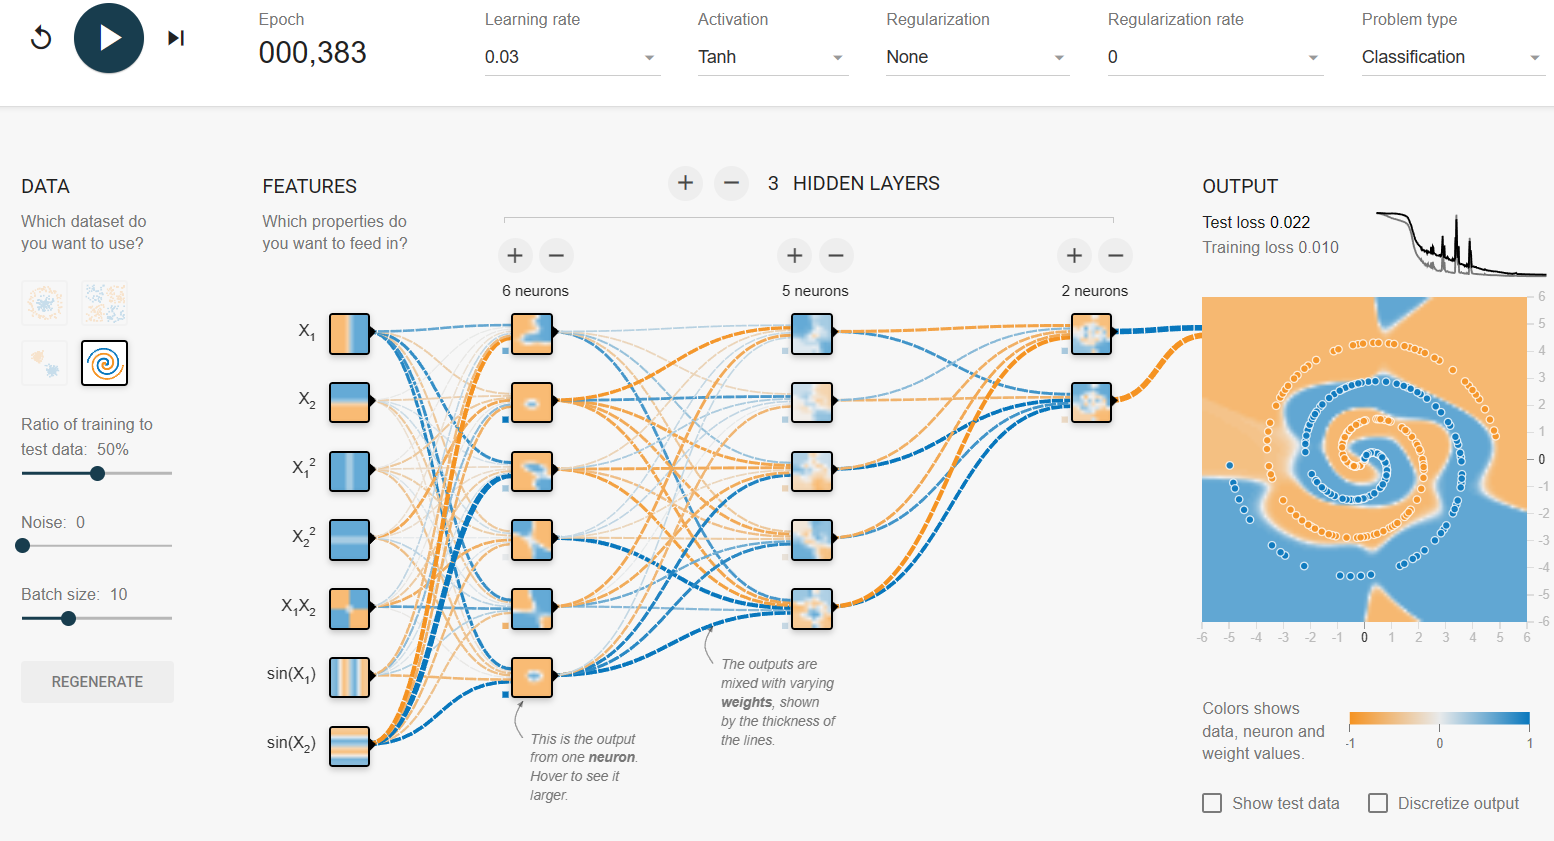
\includegraphics[width=0.8\textwidth]{figures/mlp_manual.png}
    \caption{Multi layer perceptron show the ability to  classify coordinates. We display parameters which led to good results on the spiral classification.}
    \label{fig:MPL_search}
\end{figure}

\begin{itemize}
    \item The Cybenko theorem of universal approximation states that we should be able to classify this point cloud with a single hidden layer with enough neurons. 
    \item When we use ReLu function, MLP outputs a piecewise linear function of the input coordinates.
    \item To classify the spiral points, the output logits may need to use the radius... which is possible to approximate with a very wide hidden layer.
    \item Hower instead of learning to appoximate $x^2 + y^2$ with a bunch of layers and ReLU to get the radius, we can directly inject it as an extra input.
    \item Introducing squared coordinates (and sinus embeddings) allows the model to output piecewise linear functions of more complex inputs features (a piecewise quadratic form if we consider the squared $x^2$ ).
    \item We note that finding the right architecture (depth and number of layers) is a matter of trial and error here.
\end{itemize}

We can see that eventually, we're able to find correct parameters which allow finding a shape which roughly match the spiral.   

Now the following lab session deals on how we classify 3D point clouds (e.g. unordered sets of points in 3D space). We will use a PointNet architecture to classify 3D point clouds.

\section*{Question 1}

We train our model on ModelNet40. It has 1.708M parameters. Using a learning rate of $10^{-}2$, we
are only able to reach an accuracy of $12\%$ after 75 epochs (convergence is achieved).

The accuracy of a random classifier would be $2.5\%$, so this result is not dramatic. Please note that MLP considered that the order matters here and is not \textbf{permutation invariant}. A more

However it cannot be considered a good classifier.

\begin{figure}[H]
    \centering
    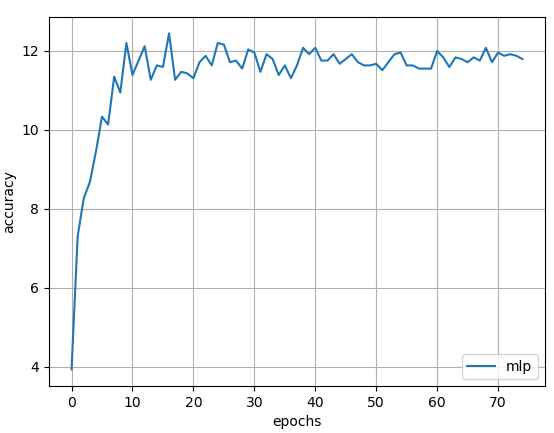
\includegraphics[width=0.5\textwidth]{figures/Q1.png}
    \caption{MLP accuracy training curve}
    \label{fig:MLP}
\end{figure}

\section*{Question 2}
On ModelNet40, we reach an accuracy of $86\%$ after 75 epochs using a learning rate of $1e-3$.
These results are considerably higher than using a simple MLP. A Pointnet without Tnets can be used
like a satisfactory classifier.
PointNet processes each point of the set separately until the max pooling operator is reached. Max pooling statisfies the permutation invariance.


\section*{Question 3}
On ModelNet40, we reach an accuracy of $84\%$ after 100 epochs using a learning rate of $5e-3$.
These results are slightly under what could be obtained without Tnet.

\section*{Question 4}
We propose two sources of data augmentation. 
\begin{itemize}
    \item First, we apply three random scaling factors centered around 1 in the x, y and z direction. 
    \item Second, we remove a random proportion of the points (around $10\%$) and replace them by duplicating other points.
\end{itemize}
Using the same parameters as before, the impact of this data augmentation is not meaningful and seems to slightly hinder the accuracy.

\end{document}


